% Version 1.0.2 DE
%
%%%%%%%%%%%%%%%%%%%%%%%%%%%%%%%%%%%%%%%%%%%%%%%%%%
%%%        			Päambel   				   %%%
%%%%%%%%%%%%%%%%%%%%%%%%%%%%%%%%%%%%%%%%%%%%%%%%%%

%%%%%%%%%%%%%%%%%%%%%%%%%%%%%%%%%%%%%%%%%%%%%%%%%%
%%%        			Päambel / Kompilieren      %%%
%%%%%%%%%%%%%%%%%%%%%%%%%%%%%%%%%%%%%%%%%%%%%%%%%%

% Wichtig:
% Um Fehler und Probleme beim Kompilieren zu vermeiden, benutzen Sie bitte immer die aktuelle Version Ihres Betriebssystems (Windows / Mac / Linux), die aktuelle Version Ihrer LaTeX-Distribution (MiKTeX / MacTeX / Tex Live) und die aktuelle Version Ihres Setzprogramms beziehungsweise LaTeX-Editors (TeXstudio / Texmaker / TeXworks / TeXnicCenter). Aktualisieren Sie Ihr Betriebssystem, Ihre LaTeX-Distribution und Ihren LaTeX-Editor vor dem Kompilieren dieser Vorlage oder lassen Sie diese von Ihrem IT-Beauftragten der Abteilung aktualisieren.
%
% Hinweise zum Kompilieren / Setzreihenfolge:
% Für die korrekte Darstellung des Layouts sowie der Bibliografien (multibib) kompilieren Sie bitte wie folgt (siehe Reihenfolge der Kompiliervorgänge):
%
%- Windows 10: über die Eingabeaufforderung PowerShell bzw. Eingabeaufforderung (cmd).
% Gehen Sie dazu in den Ordner dieses Projekts, wählen Sie keine Datei an, klicken Sie auf eine leere Stelle mit der linken Maustaste und öffnen Sie das Kontextmenü bei gedrückter Umschalttaste (Umschalttaste + rechter Mausklick) und wählen Sie "PowerShell-Fenster hier öffnen". Geben Sie anschließend "cmd" ein und rufen Sie die Kompiliervorgänge einzeln wie folgt auf (siehe Reihenfolge der Kompiliervorgänge):
%
%- macOS Big Sur 11.0.1: über das Terminal.
% Gehen Sie dazu in den Überordner dieses Projekts und wählen den Ordner an, in dem sich das Projekt befindet. Öffnen Sie nun das Kontextmenü (Sekundärklick) durch Drücken von Control+Maustaste oder beim Trackpad durch ein kurzes Tippen/Klicken mit zwei Fingern. Wählen Sie nun (Dienste)/„Neues Terminal beim Ordner“ und rufen Sie die Kompiliervorgänge einzeln wie folgt auf:
%
%
%- Reihenfolge der Kompiliervorgänge 
% pdflatex KSP_Diss_A5
% bibtex KSP_Diss_A5
% bibtex journal				% Der Dateiname der mit Bibtex auszuführenden Datei wird im Befehl "\newcites{journal}" in dieser TeX-Datei angegeben
% bibtex conference				% Der Dateiname der mit Bibtex auszuführenden Datei wird im Befehl "\newcites{conference}" in dieser TeX-Datei angegeben
% pdflatex KSP_Diss_A5
% pdflatex KSP_Diss_A5
%
%
% Fertig.
%
%
%
% Anmerkungen
%
% In TeXstudio die Kompilieraufrufe dauerhaft ändern (Windows 10, TeXstudio 3.0.1):
% Optionen/TeXstudio konfigurieren.../Erzeugen/ -> Und hier die Einträge unter "Standardcompiler" und "Standard Bibliographieprogramm" anpassen.
%
% In TeXstudio die Kompilieraufrufe manuell ausführen (Windows 10, TeXstudio 3.0.1):
% Tools/Befehle/ -> Und hier die Einträge "PDFLaTeX" und "Bibtex" (Bibtex kann jedoch nicht für bestimmte Dateien in TeXstudio ausgeführt werden, hierzu muss die Eingabeaufforderung genutzt werden s.o.).

%%%%%%%%%%%%%%%%%%%%%%%%%%%%%%%%%%%%%%%%%%%%%%%%%%
%%%        			Päambel / Documentclass    %%%
%%%%%%%%%%%%%%%%%%%%%%%%%%%%%%%%%%%%%%%%%%%%%%%%%%

% Lädt die Dokumentklasse "scrbook" (KOMA-Script-Book) mit den Eigenschaften: keine Punkte hinter der Nummerierung, Schriftgröße 10pt, Sprachpakete: englische und neue deutsche Rechtschreibung einbinden (deutsch ist Standard)
\documentclass[listof=totoc,numbers=noenddot,10pt,english,ngerman]{scrbook} 
%\documentclass[halfparskip,numbers=noenddot,a5paper,10pt,english,ngerman]{scrbook}

% \RequirePackage[ngerman=ngerman-x-latest]{hyphsubst}
% Verbesserte Silbentrennung im Deutschen nach dem aktuellen Stand

% Weitere Pakete hier einfügen
\usepackage{booktabs}
\usepackage{wrapfig}
\usepackage[all]{nowidow} % Verhindert Hurenkinder
\usepackage{amsmath}
\usepackage{amsfonts}
\usepackage{amssymb}
\usepackage{acronym}
\usepackage{trfsigns}
\usepackage{cite}
\usepackage{caption} % Für Bildunterschriften und Tabellenüberschriften
\usepackage{subcaption} % Für "subfigures"
\usepackage{enumitem}
\usepackage{calc}
\usepackage{multirow}
%\usepackage{epstopdf}
%\usepackage{url}
%\usepackage{subfigure} % old package for subfigures
%\usepackage{wrapfig}
%\providecommand\phantomsection{}
%\usepackage{color}
%\usepackage{cancel}
%\usepackage{amsthm}
%\usepackage{ulem}
%\usepackage{empheq}
%\usepackage{xcolor}
%\usepackage{float}
\usepackage{blindtext} % Blindtext zur Textdarstellung in der Vorlage ermöglichen
%\usepackage{showframe} % Seitenränder anzeigen

%%%%%%%%%%%%%%%%%%%%%%%%%%%%%%%%%%%%%%%%%%%%%%%%%%
%%%    		Präambel / Silbentrennung     	   %%%
%%%%%%%%%%%%%%%%%%%%%%%%%%%%%%%%%%%%%%%%%%%%%%%%%%

\hyphenation{
Ge-schich-te
An-ten-ne
% Worte, die nicht getrennt werden sollen, bitte ohne Bindestrich in diese Liste entragen
}

%%%%%%%%%%%%%%%%%%%%%%%%%%%%%%%%%%%%%%%%%%%%%%%%%%
%%%       Präambel /  Bibliografie			   %%%
%%%			/ Zitat / Zitieren 				   %%%
%%%			Literaturverzeichnis	   		   %%%
%%%%%%%%%%%%%%%%%%%%%%%%%%%%%%%%%%%%%%%%%%%%%%%%%%

% Zitieren aus der Bibliografie "Externe_Literatur.bib": "\cite{<ID>}"
% Zitieren aus der Bibliografie "Eigene_Journal_Papers.bib": "\citejournal{<ID>}
% Zitieren aus der Bibliografie "Eigene_Konferenz_Papers.bib": "\citeconference{<ID>}

% Standardmäßig werden alle Titel/Referenzen in den Bibliografien ausgegeben. Sollen nur die zitierten Titel/Referenzen in der Bibliografie ausgegeben werden, muss der Befehl "\nocite{*}" bzw. "\nocitejournal{*} oder "\nociteconference{*}" in der Datei ./Inhalt/Literaturverzeichnis.tex auskommentiert werden

\usepackage[resetlabels]{multibib} % Jede Bibliographie beginnt bei Zähler [1], sofern als Bibliografiestil "\bibliographiestyle{plain}" gewählt ist
%\usepackage{multibib} % Der Zähler der Bibliographien wird nicht zurückgesetzt (fortlaufende Zählung beginnend bei [1] in der Bibliografie"Journalartikel" und fortlaufend in der Bibliografie "Konferenzbeiträge"), sofern als Bibliografiestil "\bibliographiestyle{plain}" gewählt ist, bei einem anderen Bibliografiestil, z.B. "\bibliographystyle{alpha} wird kein Zähler verwendet
\newcites{journal}{Literatur/Eigene_Journal_Papers}
\newcites{conference}{Literatur/Eigene_Konferenz_Papers}
%
\usepackage{etoolbox}
\BeforeBeginEnvironment{thebibliography}{% Umdefinieren, um die eigenen Publikationen ohne Umbruch einzufügen
  \let\origchapter\chapter % save the original definition of "\chapter"
  \let\chapter\section % make \chapter behave like "\section"
}
\AfterEndEnvironment{thebibliography}{%
  \let\chapter\origchapter % restore the original definition of "\chapter"
}

%%%%%%%%%%%%%%%%%%%%%%%%%%%%%%%%%%%%%%%%%%%%%%%%%%
%%%          Präambel / Titelangaben		   %%%
%%%%%%%%%%%%%%%%%%%%%%%%%%%%%%%%%%%%%%%%%%%%%%%%%%

% pdf-Titel
\newcommand{\pdftitle}{Titel\ der\ Dissertation}

% Autor
\newcommand{\autor}{Vorname\ Nachname}

% Präambel weitestgehend ausgelagert in die Datei "dokOptions.tex"; Einbindung der Datei muss an dieser Stelle erfolgen
% Einstellungen wie Skalierung, Schriftart, Abstände sowie die Pakete "geometry", "figure", "captions" werden in der folgenden Datei verwaltet
% Version 1.1.0 DE
%
% Seitenbegrenzungen anzeigen
%\usepackage{showframe}

%%%%%%%%%%%%%%%%%%%%%%%%%%%%%%%%%%%%%%%%%%%%%%%%%%
%%% 				Informationen			  %%%%
%%%%%%%%%%%%%%%%%%%%%%%%%%%%%%%%%%%%%%%%%%%%%%%%%%

% Zeilenumbrüche manuell in \listoffigures und \listoftables setzen mit "\protect\\" (ohne Anführungszeichen) im optionalen Parameter des "\caption"-Befehls
% Beispiel: 
%\caption[Exterior view of the KIT library. Consetetur sadipscing elitr,\protect\\ sed diam nonumy eirmod tempor invidunt ut labore]{Exterior view of the KIT library. Consetetur sadipscing elitr, sed diam nonumy eirmod tempor invidunt ut labore}

% Geschütztes Leerzeichen: "~" (ohne Anführungszeichen)

%%%%%%%%%%%%%%%%%%%%%%%%%%%%%%%%%%%%%%%%%%%%%%%%%%
%%% 	Allgemeine Einstellungen			  %%%%
%%%%%%%%%%%%%%%%%%%%%%%%%%%%%%%%%%%%%%%%%%%%%%%%%%

% Seitenränder einstellen
\setlength{\topskip}{10.5pt} % Verhindern einer Fehlermeldung (Zusatz: siehe Kohm 2020: S. 36, Tabelle 2.1 "Satzspiegelmaße in Abhängigkeit von DIV bei A4 ohne Berücksichtigung von \topskip oder BCOR)

%%%%%%%%%%%%%%%%%%%%%%%%%%%%%%%%%%%%%%%%%%%%%%%%%%
%%%     	Eingabe, Ausgabe, Umlaute 		   %%%
%%%%%%%%%%%%%%%%%%%%%%%%%%%%%%%%%%%%%%%%%%%%%%%%%%

% Laden der Sprachpakete (die optionalen Parameter "ngerman" für die neue deutsche Rechtschreibung und "english" sind bereits in den optionalen Parametern der "\documentclass" gesetzt)
\usepackage{babel}

% Eingabe von Umlauten (ä, ö, ü sowie ß) durch den Parameter [utf8]
\usepackage[utf8]{inputenc}

% Ausgabe von Umlauten
\usepackage[T1]{fontenc}

%%%%%%%%%%%%%%%%%%%%%%%%%%%%%%%%%%%%%%%%%%%%%%%%%%
%%%        		Skalierung					  %%%%
%%%%%%%%%%%%%%%%%%%%%%%%%%%%%%%%%%%%%%%%%%%%%%%%%%

% Bitte skalieren Sie, entsprechend der Seitenanzahl ihres Dokuments, die Seitenränder wie folgt:

% - bis 199 Seiten (innen: 20mm, außen: 15-18mm) >>> textwidth=113mm
% - 200 bis 399 Seiten (innen: 23mm, außen: 15-18mm) >>> textwidth=110mm
% - ab 400 Seiten (innen: 25mm, außen: 15mm) >>> textwidth=108mm

%%%%%%%%%%%%%%%%%%%%%%%%%%%%%%%%%%%%%%%%%%%%%%%%%%
%%%        		Papierformat (A5)			   %%%
%%%%%%%%%%%%%%%%%%%%%%%%%%%%%%%%%%%%%%%%%%%%%%%%%%

% Seitengröße auf "a4paper" oder "a5paper" einstellbar (1. oder 2. "usepackage" wählen)
% Hinweis: Die Seitenränder für die Skalierung (s. o. "Skalierung") kann man mithilfe des Pakets "geometry" verwalten, siehe bitte hierzu die entsprechende Dokumentation unter: http://ftp.fau.de/ctan/macros/latex/contrib/geometry/geometry.pdf

% (1)
\usepackage[%
a5paper,%
headheight=1.5\baselineskip,%
top=25mm,%
inner=20mm,%
outer=15mm,%
%lines=38,%
%textwidth=113mm,%
footnotesep=7mm,%
heightrounded=true%
]{geometry}

% (2)
%\usepackage[
%a4paper,
%headheight=1.5\baselineskip,
%top=25mm,
%lines=46,
%textwidth=160mm,
%heightrounded=true,
%%bindingoffset=15mm
%]{geometry}

%\usepackage[a4paper,top=33mm,bottom=32mm,outer=25mm,inner=35mm]{geometry}

%%%%%%%%%%%%%%%%%%%%%%%%%%%%%%%%%%%%%%%%%%%%%%%%%%
%%%        			Fußzeile			   	   %%%
%%%%%%%%%%%%%%%%%%%%%%%%%%%%%%%%%%%%%%%%%%%%%%%%%%

% Abstand zwischen Textkörper und Unterkante Fußzeile (Seitenzahlen)
\setlength{\footskip}{10mm}

% Abstand zwischen Fließtext und Fußnotentrennlinie 
\setlength{\skip\footins}{20pt}

%%%%%%%%%%%%%%%%%%%%%%%%%%%%%%%%%%%%%%%%%%%%%%%%%%
%%%        		Fußnote					   	   %%%
%%%%%%%%%%%%%%%%%%%%%%%%%%%%%%%%%%%%%%%%%%%%%%%%%%

% (1) Position und Größe der Fußnoten bei 2-stelligen Fußnotennummern
\deffootnote[1.8em]{1.8em}{0em}{\makebox[1.7em][l]{\textsuperscript{\thefootnotemark\ }}}

% (2) Bitte wählen Sie für 3-stellige Fußnotennummern den folgenden Befehl und deaktivieren Sie (1), indem Sie den vorhergehenden Befehl "\deffootnote{1.7em}{0em}{\makebox[1.7em][l]{\thefootnotemark}}" auskommentieren
%\deffootnote{2.2em}{0em}{\makebox[2.2em][l]{\thefootnotemark}}

% Verhindert das Fortsetzen von Fussnoten auf der gegenüberliegenden Seite
\interfootnotelinepenalty=10000 

%%%%%%%%%%%%%%%%%%%%%%%%%%%%%%%%%%%%%%%%%%%%%%%%%%
%%%  				Absatz				  	   %%%
%%%%%%%%%%%%%%%%%%%%%%%%%%%%%%%%%%%%%%%%%%%%%%%%%%

% Zeilen auf der Seite verteilen (Es wird kein Ausgleich des unteren Seitenrandes durch Dehnung der Absatzabstände durchgeführt) 
\raggedbottom   

% Einzugtiefe (horizontaler Abstand) der ersten Zeile des Absatzes
\setlength{\parindent}{0pt}

% Vertikaler Abstand zwischen den Absätzen
\setlength{\parskip}{2.5mm}

% Schusterjungen (einzelne Zeile unten auf der Seite) unterdrücken
\clubpenalty = 10000 

% Hurenkinder (einzelne Zeile oben auf der Seite) unterdrücken
\widowpenalty = 10000
\displaywidowpenalty = 10000

% Silbentrennung am Seitenumbruch verhindern
\brokenpenalty = 10000

%%%%%%%%%%%%%%%%%%%%%%%%%%%%%%%%%%%%%%%%%%%%%%%%%%
%%%  			Gleitobjekte				   %%%
%%%			Abbildungen	Tabellen			   %%%
%%%			"{figure}", "{table}"		   	   %%%
%%%		Beschriftungen, Abstand, Caption  	   %%%
%%%%%%%%%%%%%%%%%%%%%%%%%%%%%%%%%%%%%%%%%%%%%%%%%%

\usepackage[
labelfont=bf, % Fette Beschriftungen
font=footnotesize, % Schriftgröße für Beschriftungen
]
{caption}

% Abbildungen
\captionsetup[figure]{position=below} 
\captionsetup[figure]{aboveskip=3mm} %  Abstand Bild-Bildunterschrift
\captionsetup[figure]{belowskip=-2mm} % Abstand Bildunterschrift-Fließtext

% Tabellen
% Bei der Nutzung von "\captionabove" werden die Werte "aboveskip" und "belowskip" vertauscht; bitte nutzen Sie daher den Befehl "\caption" für Tabellenüberschriften
\captionsetup[table]{position=top} 
\captionsetup[table]{aboveskip=1.5mm} % Abstand: Fließtext-Tabellenüberschrift (im PDF gemessen=~7mm) | Anmerkung: mit dem Befehl "\captionabove" ändert sich die Reihenfolge der Tabellenüberschrift  in: Tabellenüberschrift-Tabelle
\captionsetup[table]{belowskip=2.5mm} % Abstand: Tabellenüberschrift-Tabelle (im PDF gemessen=~3mm)| Anmerkung: mit dem Befehl "\captionabove" ändert sich die Reihenfolge der Tabellenüberschrift in: Fließtext-Tabellenüberschrift

% Abstand Bild: Fließtext-Bild; Bildunterschrift-Fließtext
% Abstand Tabelle: Fließtext-Tabellenüberschrift; Tabelle-Fließtext
\setlength{\intextsep}{5.5mm plus0mm minus0mm} % (im PDF gemessen für Tabellen=~7mm; für Abbildungen=~5mm)
\setlength{\textfloatsep}{7mm plus0mm minus0mm}

% Bildunterschrift Subfloats
\captionsetup[subfloat]{%
	labelformat = empty,%
	margin = 0pt,		% Einzug der Bildunterschrift von links
	%	skip = 0pt,		% Abstand zwischen Bild und Bildunterschrift
	aboveskip = 2mm,	% Abstand zwischen Bild und Bildunterschrift
	belowskip = 0mm,	% Abstand zwischen Bildunterschrift und der nächsten Bildreihe sowie zwischen Bildunterschrift und Unterschrift der Abbildung / da es hier zu einer Überschneidung der Befehle "\captionsetup[subfloat]{belowskip}" und "\captionskip[figure]{skip}" kommt, muss der vertikale Abstand zwischen den Bildreihen mit dem Befehl "\vspace{3mm}" gesetzt werden
	%	font = {footnotesize,rm},		%
	%	labelfont = {footnotesize,bf},	%
	format = hang, 		% Zweite und weitere Zeilen einrücken (an die erste ausrichten)
	indention = 0em,	% Einruecken der Beschriftung
	labelsep = space,	% "period, space, quad, newline"
	justification = RaggedRight,	% Flattersatz mit Silbentrennung
	%	justification = raggedright,	% Flattersatz ohne Silbentrennung
	%	justification = centering,	% Zentriert
	%	justification = justified,	% Blocksatz
	singlelinecheck = true, % "false" (true = bei einer Zeile immer zentrieren)
	position = auto,		% "top, bottom"
	labelformat = parens	% "simple, empty" = wie die Bezeichnung gesetzt wird
}

%%%%%%%%%%%%%%%%%%%%%%%%%%%%%%%%%%%%%%%%%%%%%%%%%%
%%%  			Gleitobjekte				   %%%
%%%			"{figure}", "{table}"		   	   %%%
%%%				Layout, Größe  	   			   %%%
%%%%%%%%%%%%%%%%%%%%%%%%%%%%%%%%%%%%%%%%%%%%%%%%%%

% Mindestfüllgrad einer Seite mit einem Gleitobjekt
\renewcommand{\floatpagefraction}{0.7}

% Maximale Größe eines Gleitobjekts am unteren Seitenrand
\renewcommand{\topfraction}{0.8}

% Maximale Größe eines Gleitobjekts am oberen Seitenrand
\renewcommand{\bottomfraction}{0.8}

% Mögliche Abstandsvergrößerung innerhalb einer Zeile bei unschönem Zeilenumbruch
\setlength{\emergencystretch}{4pt}

% Mindestanteil an Text auf einer Seite mit Gleitobjekt
\renewcommand{\textfraction}{0.1}

%%%%%%%%%%%%%%%%%%%%%%%%%%%%%%%%%%%%%%%%%%%%%%%%%%
%%%  				Zeilenabstand			   %%%
%%%%%%%%%%%%%%%%%%%%%%%%%%%%%%%%%%%%%%%%%%%%%%%%%%

% Zeilenabstände auf 1-fach festlegen
%\usepackage[singlespacing]{setspace}

% Zeilenabstände auf 1,15-fach festlegen
\usepackage{setspace}
\setstretch{1.15}

% Zeilenabstände auf 1,2-fach festlegen
%\usepackage{setspace}
%\setstretch{1.2}

% Zeilenabstände auf 1,5-fach festlegen
%\usepackage[onehalfspacing]{setspace}

%%%%%%%%%%%%%%%%%%%%%%%%%%%%%%%%%%%%%%%%%%%%%%%%%%
%%% 		Inhaltsverzeichnis		   		   %%%
%%%%%%%%%%%%%%%%%%%%%%%%%%%%%%%%%%%%%%%%%%%%%%%%%%

% Inhaltsverzeichnis richtig darstellen
\usepackage[titles]{tocloft}

% Auch bei den Kapiteln Punkte darstellen
\renewcommand{\cftchapdotsep}{\cftdotsep}
\renewcommand{\cftchapleader}{\cftdotfill{\cftchapdotsep}}

% Seitenzahlen bei Kapitel in serifenloser Schriftart darstellen
\renewcommand{\cftchappagefont}{\fontfamily{phv}\normalsize\bfseries}

% Verzeichnisse aktualisieren
%Fonts im Inhaltsverzeichnis
\renewcommand\cftchapfont{\fontfamily{phv}\normalsize\bfseries}
\renewcommand\cftsecfont{\fontfamily{phv}\fontsize{11}{11}}

%Fonts in Kapiteln und sections...
%\renewcommand\cftchappagefont{\fontfamily{phv}\normalsize\bfseries}
\renewcommand\cftsecpagefont{\fontfamily{phv}\fontsize{11}{11}}

\usepackage{makeidx}

%%%%%%%%%%%%%%%%%%%%%%%%%%%%%%%%%%%%%%%%%%%%%%%%%%
%%% 			Überschriften			  	   %%%
%%%%%%%%%%%%%%%%%%%%%%%%%%%%%%%%%%%%%%%%%%%%%%%%%%

% Auch die 4. Ebene nummerieren (subsubsection)
\setcounter{secnumdepth}{4} 

% Bis Ebene 3 (subsection) im Inhaltsverzeichnis anzeigen
\setcounter{tocdepth}{2}

% Schriftarten und -größen für die Überschriften vorgeben
\addtokomafont{chapter}{\fontfamily{phv}\fontsize{18}{20}\bfseries} 		% z. B. "2 Stand der Technik"
\addtokomafont{section}{\fontfamily{phv}\fontsize{14}{16}\bfseries}			% z. B. "2.1 Literatur und Forschung"
\addtokomafont{subsection}{\fontfamily{phv}\fontsize{12}{14}\bfseries}		% z. B. "2.1.1 Disziplinäre Entwicklung"
\addtokomafont{subsubsection}{\fontfamily{phv}\fontsize{10}{12}\bfseries}	% z. B. "2.1.1.1 Genese wissenschaftlicher" Konzepte"

%%%%%%%%%%%%%%%%%%%%%%%%%%%%%%%%%%%%%%%%%%%%%%%%%%
%%% 		Überschriften auslinieren 	   	   %%%
%%%%%%%%%%%%%%%%%%%%%%%%%%%%%%%%%%%%%%%%%%%%%%%%%%

% Horizonaler Abstand zwischen Nummerierung und Überschrift
\renewcommand*{\chapterformat}{\makebox[1.3cm][l]{\thechapter\autodot}}
\renewcommand*{\sectionformat}{\makebox[1.3cm][l]{\thesection\autodot}}
\renewcommand*{\subsectionformat}{\makebox[1.3cm][l]{\thesubsection\autodot}}
\renewcommand*{\subsubsectionformat}{\makebox[1.3cm][l]{\thesubsubsection\autodot}}

%%%%%%%%%%%%%%%%%%%%%%%%%%%%%%%%%%%%%%%%%%%%%%%%%%
%%% 	Bezeichnungen: Abbildung / Tabelle 	   %%%
%%%%%%%%%%%%%%%%%%%%%%%%%%%%%%%%%%%%%%%%%%%%%%%%%%

% Bezeichnungsnamen angeben
\addto\captionsngerman{\renewcommand{\figurename}{Abbildung}}
\addto\captionsngerman{\renewcommand{\tablename}{Tabelle}}

%%%%%%%%%%%%%%%%%%%%%%%%%%%%%%%%%%%%%%%%%%%%%%%%%%
%%% 				Schriftgröße			   %%%
%%%			Abbildungen, Kopf- Fußzeilen, 	   %%%
%%%		 	Seitenzahl,Textfarbe   	   		   %%%
%%%%%%%%%%%%%%%%%%%%%%%%%%%%%%%%%%%%%%%%%%%%%%%%%%

% Größen der Beschriftungen vorgeben
%\addtokomafont{caption}{\footnotesize}
%\setkomafont{captionlabel}{\footnotesize}

% Größe der Kopf- und Fußzeile vorgeben
\setkomafont{pageheadfoot}{\footnotesize} 

% Größe der Seitenzahl
\setkomafont{pagenumber}{\normalsize}

% Farben im Dokument zulassen
\usepackage{color}

% Textfarbe schwarz definieren
\color[cmyk]{0,0,0,1}

%%%%%%%%%%%%%%%%%%%%%%%%%%%%%%%%%%%%%%%%%%%%%%%%%%
%%% 			Schriftarten			  	   %%%
%%%%%%%%%%%%%%%%%%%%%%%%%%%%%%%%%%%%%%%%%%%%%%%%%%

%%%%%%%%%%%%%%%%%%%%%%%%%%%%%%%%%%%%%%%%%%%%%%%%%%
%%% 			Mit Serifen			  	   	   %%%
%%%%%%%%%%%%%%%%%%%%%%%%%%%%%%%%%%%%%%%%%%%%%%%%%%

% Nimbus 15 Serif
% Beispiele zum Schriftbild (Typografie)siehe: https://tug.org/FontCatalogue/nimbus15serif/
\usepackage{nimbusserif}

% URW Nimbus Roman (ähnlich Times New Roman)
% Beispiele zum Schriftbild (Typografie)siehe: https://tug.org/FontCatalogue/urwnimbusroman/ 
%\usepackage{mathptmx}

% Utopia Regular with Fourier
% Beispiele zum Schriftbild (Typografie)siehe: https://tug.org/FontCatalogue/utopia-fouriermath/ 
%\usepackage{fourier}

% Utopia Regular with Math Design
% Beispiele zum Schriftbild (Typografie)siehe: https://tug.org/FontCatalogue/utopia-mathdesign/ \usepackage[adobe-utopia]{mathdesign}

%%%%%%%%%%%%%%%%%%%%%%%%%%%%%%%%%%%%%%%%%%%%%%%%%%
%%% 			Ohne Serifen		  	   	   %%%
%%%%%%%%%%%%%%%%%%%%%%%%%%%%%%%%%%%%%%%%%%%%%%%%%%

% URW Nimbus Sans
% Beispiele zum Schriftbild (Typografie)siehe: https://tug.org/FontCatalogue/urwnimbussans/ 
%\usepackage[scaled]{helvet}
%\renewcommand*\familydefault{\sfdefault}

% Nimbus 15 Sans
% Beispiele zum Schriftbild (Typografie)siehe: https://tug.org/FontCatalogue/nimbus15sans/ 
%\usepackage{nimbussans}
%\renewcommand*\familydefault{\sfdefault}

%%%%%%%%%%%%%%%%%%%%%%%%%%%%%%%%%%%%%%%%%%%%%%%%%%
%%%        			Microtype			   	   %%%
%%%%%%%%%%%%%%%%%%%%%%%%%%%%%%%%%%%%%%%%%%%%%%%%%%
% \usepackage[stretch=10,shrink=10]{microtype} % Verhindert Unschärfe und Verschwimmen der Schrift und reduziert die Anzahl der Badboxes (underfull/overfull); muss nach der Schriftart eingebunden werden

%%%%%%%%%%%%%%%%%%%%%%%%%%%%%%%%%%%%%%%%%%%%%%%%%%
%%%        			Kopfzeile			   	   %%%
%%%%%%%%%%%%%%%%%%%%%%%%%%%%%%%%%%%%%%%%%%%%%%%%%%

% Paket für Kopf- und Fußzeilen
\usepackage[
markcase=ignoreuppercase,
automark,
autooneside=false
]{scrlayer-scrpage}
%\usepackage[nouppercase]{scrpage2} % Obsoletes Paket, das durch das Paket "\usepackage{scrlayer-scrpage}" ersetzt wurde

% Linie in der Kopfzeile definieren 
% "Das Element [headsepline] wird nach \normalfont und nach den Elementen pageheadfoot und pagehead angewandt." (Kohm 2020: 268)
\KOMAoptions{headsepline=0.5pt}
%\setheadsepline{0.5pt} % Befehlszeile für das obsolete Paket "\usepackage{scrpage2}"

% Keine Kopf/Fußzeile auf leeren Seiten
%\usepackage{emptypage} % Usage of package `emptypage' together(scrbook) with a KOMA-Script class is not recommended

% Abstand zwischen Textkörper und Linie in der Kopfzeile
\setlength{\headsep}{8mm}

%%%%%%%%%%%%%%%%%%%%%%%%%%%%%%%%%%%%%%%%%%%%%%%%%%
%%% 				Notizen		  	   	   	   %%%
%%%%%%%%%%%%%%%%%%%%%%%%%%%%%%%%%%%%%%%%%%%%%%%%%%

% Erlaubt das Einfügen von Notizen
%\usepackage{todonotes}

% Deaktiviert alle eingefügten Notizen
%\usepackage[disable]{todonotes}

% Einfügen von Notizen im Fließtext
%\todo[inline]{Das ist eine Notiz}

%%%%%%%%%%%%%%%%%%%%%%%%%%%%%%%%%%%%%%%%%%%%%%%%%%
%%% 			URLs/links					   %%%
%%%%%%%%%%%%%%%%%%%%%%%%%%%%%%%%%%%%%%%%%%%%%%%%%%

% Darstellung URLs mit Zeilenumbruch
\usepackage[hyphens]{url}

% Zeilenumbrüche in URLs nach folgenden Zeichen
\appto\UrlBreaks{\do\a\do\b\do\c\do\d\do\e\do\f\do\g\do\h\do\i\do\j\do\k\do\l\do\m\do\n\do\o\do\p\do\q\do\r\do\s\do\t\do\u\do\v\do\w\do\x\do\y\do\z\do\/\do\.}

% Darstellung und Verlinkungen im pdf-Dokument einstellen
\usepackage[hidelinks,% Links als normaler Text darstellen
%    colorlinks, % Links in Farbe darstellen
%    citecolor = blue, % Quellenangaben im Fließtext in der ausgewählten Schriftfarbe darstellen
	pdfpagemode = UseNone,% Lesezeichen im PDF-Reader nicht anzeigen
	pdfpagelayout = TwoColumnRight,% Seitenanzeige des PDF-Dokuments angeben
	pdfauthor = {\autor},% Autor des PDF-Dokuments
	pdftitle = {\pdftitle}]% Titel des PDF-Dokuments
	{hyperref}
	
%%%%%%%%%%%%%%%%%%%%%%%%%%%%%%%%%%%%%%%%%%%%%%%%%%
%%% 	Einstellungen weiterer Pakete		   %%%
%%%%%%%%%%%%%%%%%%%%%%%%%%%%%%%%%%%%%%%%%%%%%%%%%%

% Ansicht Literaturverzeichnis
%\bibliographystyle{plaindin}

% Einbinden von Bildern ermöglichen
\usepackage{graphicx}	

% Gedrehte Objekte ermöglichen
\usepackage{rotating}

% Erweiterte Tabellenumgebung
\usepackage{tabularx}

% Erweiterte Flattersatz-Kommandos
\usepackage{ragged2e}

% Linksbündiger Flattersatz in den Bezeichnungen
%\usepackage[justification=RaggedRight]{caption}
%\usepackage[justification=justified]{caption}
%\captionsetup[subfigure]{justification=RaggedRight}

% Neuer Spaltentyp "L" mit Breitenangabe für linksbündigen Flattersatz
\newcolumntype{L}[1]{>{\RaggedRight\arraybackslash}p{#1}}

% Mathematische Symbole
\usepackage{amsmath,amssymb}

% Zeilen in Tabellen können verbunden werden
\usepackage{multirow}

% Zusätzliche Textsymbole zur Verfügung stellen
\usepackage{textcomp}

% Operatorensymbole definieren
\newcommand{\real}{\operatorname{Re}}				% Realteil
\newcommand{\opdiv}{\operatorname{div}}				% Divergenzoperator
\newcommand{\rot}{\operatorname{rot}}				% Rotationsoperator
\newcommand{\grad}{\operatorname{grad}}				% Gradientenoperator
\newcommand{\imag}{\operatorname{Im}}				% Imaginärteil
\newcommand{\imein}{\operatorname{j}}				% Imaginäre Einheit "j"

% Erweiterte Listenanweisungen
\usepackage{etoolbox}

% Einzug im Abbildungsverzeichnis zu null setzen
\renewcommand{\cftfigindent}{0cm}

% Einzug im Tabellenverzeichnis zu null setzen
\renewcommand{\cfttabindent}{0cm}
	
% Deutsches Abkürzungsverzeichnis erstellen
%\usepackage[english]{nomencl}
\usepackage[german]{nomencl}

% Befehl für einen Eintrag im Abkürzungsverzeichnis in "\sym" umbennen
\let\sym\nomenclature

% Name des Abkürzungsverzeichnis ändern
\renewcommand{\nomname}{Abkürzungs- und Symbolverzeichnis}

% Spaltenbreite der Formelzeichen auf "20 %" der Textbreite setzen
\setlength{\nomlabelwidth}{.2\textwidth}

% Einheiten in die Bezeichnung mit aufnehmen und rechtsbündig setzen
\newcommand{\nomunit}[1]{\renewcommand{\nomentryend}{\hspace*{\fill}#1}}

% Zeilenabstände verkleineren auf normalen Textabstand
\setlength\nomitemsep{-\parsep}

% Abkürzungsverzeichnis erzeugen
\makenomenclature

% Weitere Verzeichnisse erzeugen
\makeindex

\AtBeginDocument{ % 
  \newcaptionname{ngerman}\equationname{Formel} % 
  \newcaptionname{ngerman}\listequationname{Formelverzeichnis} % 
  \addtocontents{toc}{\protect\activateonlyattoc} % Z. B. für Umbrüche von langen Überschriften im Inhaltsverzeichnis mit dem Befehl \onlyattoc{\protect\\} (Beispiel: \chapter{Lange Kapitelüberschriften und der manuelle Zeilenumbruch \onlyattoc{\protect\\} für eine saubere Darstellung im Text})
}

\DeclareRobustCommand*{\onlyattoc}[1]{} % Z. B. für Umbrüche von langen Überschriften im Inhaltsverzeichnis mit dem Befehl \onlyattoc{\protect\\} (Beispiel: \chapter{Lange Kapitelüberschriften und der manuelle Zeilenumbruch \onlyattoc{\protect\\} für eine saubere Darstellung im Text})
\newcommand*{\activateonlyattoc}{\DeclareRobustCommand*{\onlyattoc}[1]{##1}}% Z. B. für Umbrüche von langen Überschriften im Inhaltsverzeichnis mit dem Befehl \onlyattoc{\protect\\} (Beispiel: \chapter{Lange Kapitelüberschriften und der manuelle Zeilenumbruch \onlyattoc{\protect\\} für eine saubere Darstellung im Text})

\DeclareNewTOC[ 
  tocentryindent=0pt,
  tocentrynumwidth=2em,
  type=equation,
  name={Gl.}, 
  types=equations, 
  listname={Formelverzeichnis}, 
]{equ} 
\newcommand{\equationentry}[2][\theequation]{ % 
  \addxcontentsline{equ}{equation}[{#1}]{\kern 1em #2} % 
} 
\BeforeStartingTOC[equ]{\def\autodot{:}}



% Literaturverzeichnis
%-----------------------
%
% Kohm 2020: Kohm, Markus; Neukamp, Frank; Kielhorn, Axel (2020): Die Anleitung. KOMA-Script. Markus Kohm. 2020-03.12. (Online)

% Titel
\newcommand{\headtitle}{Titel der Dissertation}

%\makeindex

\newcommand{\nauthor}{Vorname Nachname}
\newcommand{\akadtitel}{M.Sc.}
\newcommand{\geburtsort}{Geburtsort}

\newcommand{\ntitle}{Titel der Dissertation}

\newcommand{\referent}{Prof. Dr.-Ing. Hauptreferent}
\newcommand{\korreferent}{Prof. Dr.-Ing. Korreferent}
\newcommand{\ndatum}{tt.mm.jjjj}

%\renewcommand{\figurename}{Abbildung}
%\renewcommand{\tablename}{Tabelle}

%\ohead[]{}
%\ofoot[\pagemark]{\pagemark} % Seitenzahlen unten außen

%\ihead[]{}
%\ohead[]{\headmark} % Kopfzeilen oben außen

%%%%%%%%%%%%%%%%%%%%%%%%%%%%%%%%%%%%%%%%%%%%%%%%%%
%%%				Begin Dokument				   %%%
%%%%%%%%%%%%%%%%%%%%%%%%%%%%%%%%%%%%%%%%%%%%%%%%%%

\begin{document}

%%%%%%%%%%%%%%%%%%%%%%%%%%%%%%%%%%%%%%%%%%%%%%%%%%
%%%				Dokument / Layout			   %%%
%%%%%%%%%%%%%%%%%%%%%%%%%%%%%%%%%%%%%%%%%%%%%%%%%%

% Voreingestellter Seitenstil verwenden
\pagenumbering{gobble}

% Römische Seitennummerierung verwenden
\pagestyle{scrheadings}

% Setzt Kapitelüberschrift auch auf rechte Seite der Kopfzeile, da keine Unterkapitel
\renewcommand{\chaptermark}[1]{\markboth{\thechapter\ \  #1}{\thechapter\ \  #1}} 

% Seitenzahl mit 5 beginnen (KSP setzt 4 beschriftete Seiten davor)
%\setcounter{page}{5}

%%%%%%%%%%%%%%%%%%%%%%%%%%%%%%%%%%%%%%%%%%%%%%%%%%
%%%				Titelblatt (include)		   %%%
%%%%%%%%%%%%%%%%%%%%%%%%%%%%%%%%%%%%%%%%%%%%%%%%%%

\begin{titlepage}
\vspace*{0em}
\begin{center}

\begin{doublespace}
	{\LARGE \textbf{\ntitle}}
\end{doublespace}

		\vskip 2em
	Zur Erlangung des akademischen Grades eines 
		\vskip 1em
	{\large\textbf{DOKTOR-INGENIEURS}} 
		\vskip 2em
	von der Fakult\"at f\"ur \\
	Elektrotechnik und Informationstechnik,\\
	des Karlsruher Instituts f\"ur Technologie (KIT) 
		\vskip 1em
	genehmigte%vorgelegte
		\vskip 1em
	{\large \textbf{DISSERTATION}} \\
		\vskip 1em
	von 
		\vskip 1em
	{\large\textbf{\akadtitel{} \nauthor}} \\
		\vskip 0.25em
	geb. in \geburtsort
\end{center}

\vfill
\begin{center}

\begin{tabular*}{1.02\textwidth}[h]{@{\extracolsep{\fill}}ll}
Tag der m\"undlichen Pr\"ufung: & 26.06.2019 \\
Hauptreferent: & \referent \\
Korreferent: & \korreferent
\end{tabular*}

\end{center}

\end{titlepage}

%%%%%%%%%%%%%%%%%%%%%%%%%%%%%%%%%%%%%%%%%%%%%%%%%%
%%%			Titelteil / Kapitel (include)	   %%%
%%%%%%%%%%%%%%%%%%%%%%%%%%%%%%%%%%%%%%%%%%%%%%%%%%

% Titelteil; Kapitel im Titelteil erhalten keine Kapitelnummer im Inhaltsverzeichnis
\frontmatter 

% Zusammenfassung
\markboth{Zusammenfassung}{Zusammenfassung}
\chapter*{Zusammenfassung}
\label{cha:Zusammenfassung}
\addcontentsline{toc}{chapter}{Zusammenfassung}

%%%%%%%%%%%%%%%%%%%%%%%%%%%%%%%%%%%%%%%%%%%%%%%%%%

\Blindtext[6]

Lorem ipsum dolor sit amet, consetetur sadipscing elitr, sed diam nonumy eirmod tempor invidunt ut labore et dolore magna aliquyam erat, sed diam voluptua. At vero eos et accusam et justo duo dolores et ea rebum. Stet clita kasd gubergren, no sea takimata sanctus est Lorem ipsum dolor sit amet. Lorem ipsum dolor sit amet, consetetur sadipscing elitr, sed diam nonumy eirmod tempor invidunt ut labore et dolore magna aliquyam erat, sed diam voluptua. At vero eos et accusam et justo duo dolores et ea rebum. Stet clita kasd gubergren, no sea takimata sanctus est Lorem ipsum dolor sit amet.

% Vorwort
\markboth{Vorwort}{Vorwort}
\chapter*{Vorwort}
\label{cha:Vorwort}
\addcontentsline{toc}{chapter}{Vorwort}

%%%%%%%%%%%%%%%%%%%%%%%%%%%%%%%%%%%%%%%%%%%%%%%%%%

\Blindtext[6]

Lorem ipsum dolor sit amet, consetetur sadipscing elitr, sed diam nonumy eirmod tempor invidunt ut labore et dolore magna aliquyam erat, sed diam voluptua. At vero eos et accusam et justo duo dolores et ea rebum. Stet clita kasd gubergren, no sea takimata sanctus est Lorem ipsum dolor sit amet. Lorem ipsum dolor sit amet, consetetur sadipscing elitr, sed diam nonumy eirmod tempor invidunt ut labore et dolore magna aliquyam erat, sed diam voluptua. At vero eos et accusam et justo duo dolores et ea rebum. Stet clita kasd gubergren, no sea takimata sanctus est Lorem ipsum dolor sit amet.

% Inhaltsverzeichnis \tableofcontents (siehe Inhaltsverzeichnis.tex)
\markboth{Inhaltsverzeichnis}{Inhaltsverzeichnis}

% \renewcommand\cftdotsep{4.621757}  % Bei größeren Werten wird der letzte Punkt nicht mehr gezeichnet, weil er "außerhalb der Zeile" liegt (erfordert das Paket "\usepackage{tocloft}")

% \pdfbookmark{\contentsname}{toc} % Name des Inhaltsverzeichnisses "Contents im PDF-Dokument" (erfordert das Paket "\usepackage{bookmark}")
\cleardoublepage\pdfbookmark{Inhaltsverzeichnis}{toc} % Name des Inhaltsverzeichnisses "Inhaltsverzeichnis" im PDF-Dokument (erfordert das Paket "\usepackage{bookmark}")
% \pdfbookmark{Inhaltsverzeichnis}{toc} % Name des Inhaltsverzeichnisses "Inhaltsverzeichnis" im PDF-Dokument (erfordert das Paket "\usepackage{bookmark}")
\renewcommand{\contentsname}{Inhaltsverzeichnis} % Ändert die Überschrift und das Lesezeichen in der PDF-Datei von "Contents" in "Inhaltsverzeichnis"; dieser Befehl ist Lokalitätsgebunden
\tableofcontents

%%%%%%%%%%%%%%%%%%%%%%%%%%%%%%%%%%%%%%%%%%%%%%%%%%


% Abkürzungen und Symbole
\markboth{Abk\"urzungen und Symbole}{Abk\"urzungen und Symbole}
\chapter*{Abkürzungen und Symbole}
\label{cha:Abkuerzungen_Symbole}
\addcontentsline{toc}{chapter}{Abkürzungen und Symbole}

%%%%%%%%%%%%%%%%%%%%%%%%%%%%%%%%%%%%%%%%%%%%%%%%%%

\subsubsection*{Abkürzungen}
\markboth{Abk\"urzungen und Symbole}{Abk\"urzungen und Symbole}
%\begin{spacing}{0.9}	% Eventuell ändern, um eine schönere Seitendarstellung zu erhalten
%\begin{acronym}[XXXXXXX]
%\setlength{\itemsep}{0.0585cm}
%\begingroup
%\acro{IHE}{Institut f\"ur Hochfrequenztechnik und Elektronik}
%\acro{KIT}{Karlsruher Institut f\"ur Technologie}
%\endgroup
%\end{acronym}
%\end{spacing}
\begin{description}[leftmargin=\widthof{\textbf{XXXXXXX}\hspace{\labelsep}},style=nextline]
	\item[$\mathbf{IHE}$] Institut f\"ur Hochfrequenztechnik und Elektronik
	\item[$\mathbf{KIT}$] Karlsruher Institut f\"ur Technologie
\end{description}

%%%%%%%%%%%%%%%%%%%%%%%%%%%%%%%%%%%%%%%%%%%%%%%%%%

\subsubsection*{Konstanten}
\begin{description}[leftmargin=\widthof{\textbf{XXXXXXX}\hspace{\labelsep}},style=nextline]
	\item[$\pi$] Kreiszahl Pi: $3$,$14159\ldots$
\end{description}

%%%%%%%%%%%%%%%%%%%%%%%%%%%%%%%%%%%%%%%%%%%%%%%%%%

\subsubsection*{Lateinische Symbole und Variablen}

\begin{description}[leftmargin=\widthof{\textbf{XXXXXXX}\hspace{\labelsep}},style=nextline]
	\item[$\mathbf{B}$] Strahlformungsmatrix
	\item[$B$] Bandbreite
	\item[$f$] Frequenz
	\item[$g$] Gewichtungsfaktor
\end{description}


%%%%%%%%%%%%%%%%%%%%%%%%%%%%%%%%%%%%%%%%%%%%%%%%%%

%\clearpage

\subsubsection*{Griechische Symbole und Variablen}
\begin{description}[leftmargin=\widthof{\textbf{XXXXXXX}\hspace{\labelsep}},style=nextline]
	\item[$\lambda$] Wellenl\"ange
	\item[$\varphi$] Phasenverschiebung
\end{description}
%%%%%%%%%%%%%%%%%%%%%%%%%%%%%%%%%%%%%%%%%%%%%%%%%%

\subsubsection*{Operatoren und mathematische Symbole}
\begin{description}[leftmargin=\widthof{\textbf{XXXXXXX}\hspace{\labelsep}},style=nextline]
	\item[$a$] komplexe Gr\"o{\ss}e
	\item[$\vec a$] komplexer Vektor
	%& && & &&
\end{description}

%%%%%%%%%%%%%%%%%%%%%%%%%%%%%%%%%%%%%%%%%%%%%%%%%%

\subsubsection*{Allgemeine Tiefindizes}
\begin{description}[leftmargin=\widthof{\textbf{XXXXXXX}\hspace{\labelsep}},style=nextline]
	\item[$\mathrm{adapt}$] adaptiv
	\item[$\mathrm{incoh}$] inkohärent
\end{description}


% Jedes neue Kapitel beginnt auf der rechten Seite
\cleardoublepage 

%%%%%%%%%%%%%%%%%%%%%%%%%%%%%%%%%%%%%%%%%%%%%%%%%%
%%%				Hauptteil / Layout			   %%%
%%%%%%%%%%%%%%%%%%%%%%%%%%%%%%%%%%%%%%%%%%%%%%%%%%

% Römische Seitennummerierung verwenden
\pagenumbering{roman} 
\setcounter{page}{1}

% Hauptteil; Kapitel im Hauptteil werden mit Zahlen nummeriert im Inhaltsverzeichnis
\mainmatter 

% Zeilenabstand innerhalb Tabellen (urspruenglich 1,4)
\renewcommand{\arraystretch}{1.2} 

% Abstand zwischen Spalten in Tabellen
\setlength{\tabcolsep}{1mm} 

% Abstände bei Aufzählungspunkten
\setlist[itemize]{itemsep=0mm, topsep=1mm} 

% Arabische Seitennummerierung verwenden
\pagenumbering{arabic} 

%\RedeclareSectionCommand[beforeskip=-1.00\baselineskip,afterskip=0.50\baselineskip]{section}
%\RedeclareSectionCommand[beforeskip=-0.75\baselineskip,afterskip=0.50\baselineskip]{subsection}
%\RedeclareSectionCommand[beforeskip=-0.50\baselineskip,afterskip=0.25\baselineskip]{subsubsection}

%%%%%%%%%%%%%%%%%%%%%%%%%%%%%%%%%%%%%%%%%%%%%%%%%%
%%%			Hauptteil / Kapitel (include)	   %%%
%%%%%%%%%%%%%%%%%%%%%%%%%%%%%%%%%%%%%%%%%%%%%%%%%%

% Einleitung und Motivation
\markboth{Einleitung und Motivation}{Einleitung und Motivation}

\chapter{Einleitung und Motivation (automatische Einrückung \mbox{im Inhaltsverzeichnis})}
\label{cha:Einleitung und Motivation}
Lorem ipsum dolor sit amet, consetetur sadipscing elitr, sed diam nonumy eirmod tempor invidunt ut labore et dolore magna aliquyam erat, sed diam voluptua. At vero eos et accusam et justo duo dolores et ea rebum. Stet clita kasd gubergren, no sea takimata sanctus est Lorem ipsum dolor sit amet. Lorem ipsum dolor sit amet, consetetur sadipscing elitr, sed diam nonumy eirmod tempor invidunt ut labore et dolore magna aliquyam erat, sed diam voluptua. At vero eos et accusam et justo duo dolores et ea rebum. Stet clita kasd gubergren, no sea takimata sanctus est Lorem ipsum dolor sit amet.

\section{Einleitung}
\label{sec:Einleitung}
Lorem ipsum dolor sit amet, consetetur sadipscing elitr, sed diam nonumy eirmod tempor invidunt ut labore et dolore magna aliquyam erat, sed diam voluptua. At vero eos et accusam et justo duo dolores et ea rebum. Stet clita kasd gubergren, no sea takimata sanctus est Lorem ipsum dolor sit amet. Lorem ipsum dolor sit amet, consetetur sadipscing elitr, sed diam nonumy eirmod tempor invidunt ut labore et dolore magna aliquyam erat, sed diam voluptua. At vero eos et accusam et justo duo dolores et ea rebum. Stet clita kasd gubergren, no sea takimata sanctus est Lorem ipsum dolor sit amet.

\section{Motivation}
\label{sec:Motivation}
Lorem ipsum dolor sit amet, consetetur sadipscing elitr, sed diam nonumy eirmod tempor invidunt ut labore et dolore magna aliquyam erat, sed diam voluptua. At vero eos et accusam et justo duo dolores et ea rebum. Stet clita kasd gubergren, no sea takimata sanctus est Lorem ipsum dolor sit amet. Lorem ipsum dolor sit amet, consetetur sadipscing elitr, sed diam nonumy eirmod tempor invidunt ut labore et dolore magna aliquyam erat, sed diam voluptua. At vero eos et accusam et justo duo dolores et ea rebum. Stet clita kasd gubergren,\footnote{Asimporro modi dis accusci istiis volorrovit, voluptam quisquas ipsuntios elenim nonecto quo cus quis es dolut re omnim qui occum voloriatus et ratus quis ea dolorionsed estrum et dit am es doloriassus.} no sea takimata sanctus est Lorem ipsum dolor sit amet. Lorem ipsum dolor sit amet, consetetur sadipscing elitr, sed diam nonumy eirmod tempor invidunt ut labore et dolore magna aliquyam erat, sed diam voluptua:

\begin{itemize}
\item[$\bullet$] \raggedright Aufzählungen mit weniger als drei Zeilen stehen im Flattersatz. Der Befehl \verb+\raggedright+ nach \verb+\item+ erzeugt einen Flattersatz.
\item[$\bullet$] \justifying Aufzählungen mit drei oder mehr Zeilen stehen im Blocksatz. Mit dem Befehl \verb+\justifying+ nach dem Befehl \verb+\item+ kann der Absatz als Blocksatz formatiert werden. Damit passt sich der Absatz optisch an den Fließtext an und erzeugt dadurch ein kohärentes Textbild.
\item[$\bullet$] Bulletpoint 3
\item[$\bullet$] Bulletpoint 4
\item[$\bullet$] Bulletpoint 5
\end{itemize}

Lorem ipsum dolor sit amet, consetetur sadipscing elitr, sed diam nonumy eirmod tempor invidunt ut labore et dolore magna aliquyam erat, sed diam voluptua. At vero eos et accusam et justo duo dolores et ea rebum. Stet clita kasd gubergren, no sea takimata sanctus est Lorem ipsum dolor sit amet. Lorem ipsum dolor sit amet, consetetur sadipscing elitr, sed diam nonumy eirmod tempor invidunt ut labore et dolore magna aliquyam erat, sed diam voluptua. At vero eos et accusam et justo duo dolores et ea rebum. Stet clita kasd gubergren, no sea takimata sanctus est Lorem ipsum dolor sit amet.

Lorem ipsum dolor sit amet, consetetur sadipscing elitr, sed diam nonumy eirmod tempor invidunt ut labore et dolore magna aliquyam erat, sed diam voluptua. At vero eos et accusam et justo duo dolores et ea rebum. Stet clita kasd gubergren, no sea takimata sanctus est Lorem ipsum dolor sit amet. Lorem ipsum dolor sit amet, consetetur sadipscing elitr, sed diam nonumy eirmod tempor invidunt ut labore et dolore magna aliquyam erat, sed diam voluptua.\footnote{Litati dolorehendam faceperia sunt ped quas et il et voluptae perum faci dia incimpe cuptati di dolo modi bearciur, aut et, omnimus dolores tiatatem acculla ndestec turion exerund icillab.}

Lorem ipsum dolor sit amet, consetetur sadipscing elitr, sed diam nonumy eirmod tempor invidunt ut labore et dolore magna aliquyam erat, sed diam voluptua. At vero eos et accusam et justo duo dolores et ea rebum. Stet clita kasd gubergren, no sea takimata sanctus est Lorem ipsum dolor sit amet. Lorem ipsum dolor sit amet, consetetur sadipscing elitr, sed diam nonumy eirmod tempor invidunt ut labore et dolore magna aliquyam erat, sed diam voluptua. At vero eos et accusam et justo duo dolores et ea rebum. Stet clita kasd gubergren, no sea takimata sanctus est Lorem ipsum dolor sit amet

Lorem ipsum dolor sit amet, consetetur sadipscing elitr, sed diam nonumy eirmod tempor invidunt ut labore et dolore magna aliquyam erat, sed diam voluptua. At vero eos et accusam et justo duo dolores et ea rebum. Stet clita kasd gubergren, no sea takimata sanctus est Lorem ipsum dolor sit amet. Lorem ipsum dolor sit amet, consetetur sadipscing elitr, sed diam nonumy eirmod tempor invidunt ut labore et dolore magna aliquyam erat, sed diam voluptua.

% Stand der Technik
\markboth{Stand der Technik}{Stand der Technik}
\chapter{Stand der Technik (Silbentrennung im Inhaltsverzeichnis \mbox{ist deaktiviert})}
\label{cha:Stand der Technik}

%%%%%%%%%%%%%%%%%%%%%%%%%%%%%%%%%%%%%%%%%%%%%%%%%%

\section{Literatur und Forschung}
\label{sec:Literatur und Forschung}
Lorem ipsum \citet{Bucher2021, Zeitschriftler2000} dolor sit amet, consetetur sadipscing elitr, sed diam nonumy eirmod tempor invidunt ut labore et dolore magna aliquyam erat, sed diam voluptua. At vero eos et accusam et justo duo dolores et ea rebum. Stet clita kasd gubergren, no sea takimata sanctus est Lorem ipsum dolor sit amet. Lorem ipsum dolor sit amet, consetetur sadipscing elitr, sed diam nonumy eirmod tempor invidunt ut labore et dolore magna aliquyam erat, sed diam voluptua. At vero eos et accusam et justo duo dolores et ea rebum. \glqq Stet clita kasd gubergren, no sea takimata sanctus est Lorem ipsum dolor sit amet.\grqq~\citepjournal[S. 59]{Mustermann2000}

\subsection{Disziplinäre Entwicklung}
\label{ssec:Disziplinäre Entwicklung}
%Lorem ipsum dolor sit amet, consetetur sadipscing elitr, sed diam nonumy eirmod tempor invidunt ut labore et dolore magna aliquyam erat, sed diam voluptua. At vero eos et accusam et justo duo dolores et ea rebum. Stet clita kasd gubergren, no sea takimata sanctus est Lorem ipsum dolor sit amet. Lorem ipsum dolor sit amet, consetetur sadipscing elitr, sed diam nonumy eirmod tempor invidunt ut labore et dolore magna aliquyam erat, sed diam voluptua. At vero eos et accusam et justo duo dolores et ea rebum. Stet clita kasd gubergren, no sea takimata sanctus est Lorem ipsum dolor sit amet.

\subsubsection{Genese wissenschaftlicher Konzepte}
\label{sssec:Genese wissenschaftlicher Konzepte}
Lorem ipsum dolor sit amet, consetetur sadipscing elitr, sed diam nonumy eirmod tempor invidunt ut labore et dolore magna aliquyam erat, sed diam voluptua. At vero eos et accusam et justo duo dolores et ea rebum. Stet clita kasd gubergren, no sea takimata sanctus est Lorem ipsum dolor sit amet. Lorem ipsum dolor sit amet, consetetur sadipscing elitr, sed diam nonumy eirmod tempor invidunt ut labore et dolore magna aliquyam erat, sed diam voluptua. At vero eos et accusam et justo duo dolores et ea rebum. Stet clita kasd gubergren, no sea takimata sanctus est Lorem ipsum dolor sit amet.

Lorem ipsum dolor sit amet, consetetur sadipscing elitr, sed diam nonumy eirmod tempor invidunt ut labore et dolore magna aliquyam erat, sed diam voluptua. At vero eos et accusam et justo duo dolores et ea rebum. Stet clita kasd gubergren, no sea takimata sanctus est Lorem ipsum dolor sit amet. Lorem ipsum dolor sit amet, consetetur sadipscing elitr, sed diam nonumy eirmod tempor invidunt ut labore et dolore magna aliquyam erat, sed diam voluptua. At vero eos et accusam et justo duo dolores et ea rebum. Stet clita kasd gubergren, no sea takimata sanctus est Lorem ipsum dolor sit amet.\footnote{
	Erster Absatz: Diese Fußnote besitzt eine einstellige Fußnotennummer mit festem Abstand zwischen Fußnotennummer und Fußnotentext. Diese Fußnote geht über zwei Zeilen.
	
	Zweiter Absatz: Die Einzugtiefe des zweiten Absatzes ist identisch mit der Einzugtiefe des ersten Absatzes.
} % Ende der Fußnote

\subsubsection*{Zwischenüberschrift}
\label{sssec:Zwischenüberschrift}
Lorem ipsum dolor sit amet, consetetur sadipscing elitr, sed diam nonumy eirmod tempor invidunt ut labore et dolore magna aliquyam erat, sed diam voluptua.At vero eos et accusam et justo duo dolores et ea rebum. Stet clita kasd gubergren, no sea takimata sanctus est Lorem ipsum dolor sit amet. Lorem ipsum dolor sit amet, consetetur sadipscing elitr, sed diam nonumy eirmod tempor invidunt ut labore et dolore magna aliquyam erat, sed diam voluptua. At vero eos et accusam et justo duo dolores et ea rebum. Stet clita kasd gubergren, no sea takimata sanctus est Lorem ipsum dolor sit amet.\footnote[13]{
	Diese Fußnote besitzt eine zweistellige Fußnotennummer mit festem Abstand zwischen Fußnotennummer und Fußnotentext (gerundet 2 mm). Auch diese Fußnote geht über zwei Zeilen. Auch in dieser Fußnote würde es keinen Einzug eines zweiten Absatzes geben. 
	
	Falls Sie dreistellige Fußnoten nutzen, passen Sie bitte den LaTeX-Befehl unter dem Punkt „Fußnoten“ in der Datei „dokOptions\_A5.tex“ an.
} % Ende der Fußnote

Lorem ipsum dolor sit amet, consetetur sadipscing elitr, sed diam nonumy eirmod tempor invidunt ut labore et dolore magna aliquyam erat, sed diam voluptua. At vero eos et accusam et justo duo dolores et ea rebum. Stet clita kasd gubergren, no sea takimata sanctus est Lorem ipsum dolor sit amet.

%\newpage
%\setcounter{figure}{13}
\begin{figure}[h] % "\begin{figure}" ist eine Umgebung für Gleitobjekte, damit die Abbildung nummeriert und beschriftet ("\caption{}")und mit einem Label ("\label{fig:bib}") versehen und darauf verwiesen werden kann ("\ref{fig:bib}")
	\centering
	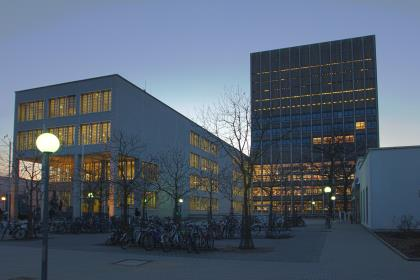
\includegraphics[width=\textwidth]{Abbildungen/bib.jpg}
	\caption{Außenansicht der KIT-Bibliothek. Bilder bitte immer manuell mit dem Parameter [h] setzen.	An dieser Stelle ist das Bild mit dem Figure-Parameter [h] platziert worden. Vor und nach der Figure-Umgebung steht eine Leerzeile.}
	\label{fig:bib}
\end{figure}

Lorem ipsum dolor sit amet, consetetur sadipscing elitr, sed diam nonumy eirmod tempor invidunt ut labore et dolore magna aliquyam erat, sed diam voluptua. At vero eos et accusam et justo duo dolores et ea rebum. Stet clita kasd gubergren, no sea takimata sanctus est Lorem ipsum dolor sit amet. Lorem ipsum dolor sit amet, consetetur sadipscing elitr, sed diam nonumy eirmod tempor invidunt ut labore et dolore magna aliquyam erat, sed diam voluptua. At vero eos et accusam et justo duo dolores et ea rebum. Stet clita kasd gubergren, no sea takimata sanctus est Lorem ipsum dolor sit amet.

Lorem ipsum dolor sit amet, consetetur sadipscing elitr, sed diam nonumy eirmod tempor invidunt ut labore et dolore magna aliquyam erat, sed diam voluptua. At vero eos et accusam et justo duo dolores et ea rebum. Stet clita kasd gubergren, no sea takimata sanctus est Lorem ipsum dolor sit amet. 	

%\newpage
\begin{figure}[h] % "\begin{figure}" ist eine Umgebung für Gleitobjekte, damit die Abbildung nummeriert und beschriftet ("\caption{}")und mit einem Label ("\label{fig:bib}") versehen und darauf verwiesen werden kann ("\ref{fig:bib}")
	\centering
%\hspace{-7pt} % Horizontale verschiebung der Bildreihe
	\subfloat[Subfloat. Bild Nr. 1. Zweizeilige Bildunterschriften stehen im Flattersatz.]{%
		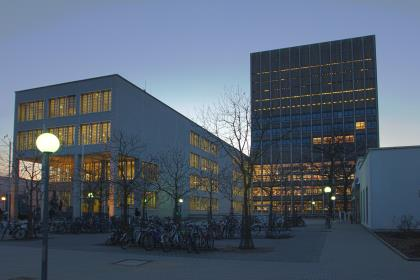
\includegraphics[width=0.49\linewidth]{Abbildungen/bib.jpg}%
	}
\hfill % Füllt den den vertikalen Abstand zwischen den Bildern auf, sofern die Bilder entsprechend klein sind
	\subfloat[Subfloat. Bild Nr. 2.]{%
		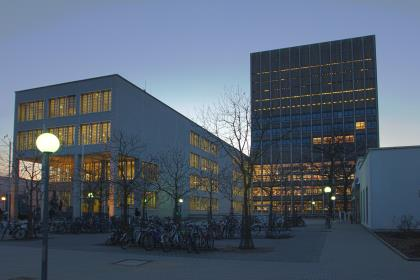
\includegraphics[width=0.49\linewidth]{Abbildungen/bib.jpg}%
	}
\\ \vspace{3mm} % Abstand zur zweiten Bildreihe % Plus Abstand aufgrund des Befehles "\captionsetup[subfloat]{belowskip=}" aus der Datei dokOptions.tex
%\hspace{-7pt} % Horizontale verschiebung der Bildreihe
	\subfloat[Subfloat. Bild Nr. 3. Mit linebreak \linebreak für einen manuellen Zeilenumbruch]{%
		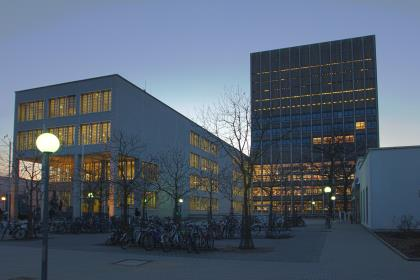
\includegraphics[width=0.49\linewidth]{Abbildungen/bib.jpg}%
	}
\hfill % Füllt den den vertikalen Abstand zwischen den Bildern auf, sofern die Bilder entsprechend klein sind
	\subfloat[Subfloat. Bild Nr. 4.]{%
		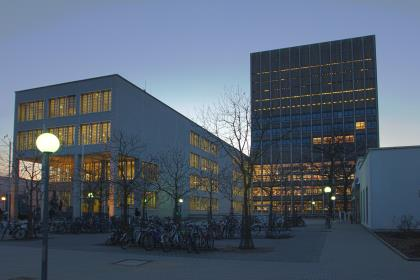
\includegraphics[width=0.49\linewidth]{Abbildungen/bib.jpg}%
	}
	\caption{Außenansicht der KIT-Bibliothek. Bilder bitte immer manuell mit dem Parameter [h] setzen.	An dieser Stelle ist das Bild mit dem Figure-Parameter [h] platziert worden. Vor und nach der Figure-Umgebung steht eine Leerzeile.}
	\label{fig:bib4}
\end{figure}

Lorem ipsum dolor sit amet, consetetur sadipscing elitr, sed diam nonumy eirmod tempor invidunt ut labore et dolore magna aliquyam erat, sed diam voluptua. At vero eos et accusam et justo duo dolores et ea rebum. Stet clita kasd gubergren, no sea takimata sanctus est Lorem ipsum dolor sit amet.

Curabitur a felis in nunc fringilla tristique. Morbi mattis ullamcorper velit. Phasellus gravida semper nisi. Nullam vel sem. Pellentesque libero tortor, tincidunt et, tincidunt eget, semper nec, quam. Sed hendrerit. Morbi ac felis. Nunc egestas, augue at pellentesque laoreet, felis eros vehicula leo, at malesuada velit leo quis pede. Donec interdum, metus et hendrerit aliquet, dolor diam sagittis ligula, eget egestas libero turpis vel mi. Nunc nulla. Fusce risus nisl, viverra et, tempor et.Pellentesque ut neque. Pellentesque habitant morbi tristique senectus et netus et malesuada fames ac turpis egestas. In dui magna, posuere eget, vestibulum et, tempor auctor, justo. In ac felis quis tortor malesuada pretium. Pellentesque auctor neque nec urna. Proin sapien ipsum, porta a, auctor quis, euismod ut, mi.

Aenean viverra rhoncus pede. Pellentesque habitant morbi tristique senectus et netus et malesuada fames ac turpis egestas. Ut non enim eleifend felis pretium feugiat vivamus quis mi. Phasellus a est. Phasellus magna. In hac habitasse platea dictumst. Curabitur at lacus ac velit ornare lobortis.\footnote{Cabo. Facerfe rferspient que nus molora doleserem. Ut a si autemo tectaquame enihil intota sam am ditati omnihil ma sequis re, aut fugiam earchil luptaque consequ.} Curabitur a felis in nunc fringilla tristique. Morbi mattis ullamcorper velit. Phasellus gravida semper nisi. Nullam vel sem. Pellentesque libero tortor, tincidunt et, tincidunt eget, semper nec, quam. Sed hendrerit.

%\newpage
Pellentesque habitant morbi tristique senectus et netus et malesuada fames ac turpis egestas. In dui magna, posuere eget, vestibulum et, tempor auctor, justo. In ac felis quis tortor malesuada pretium. Pellentesque auctor neque nec urna. Proin sapien ipsum, porta a, auctor quis, euismod ut, mi. Aenean viverra rhoncus pede. Pellentesque habitant morbi tristique senectus et netus et malesuada fames ac turpis egestas. Ut non enim eleifend felis pretium feugiat vivamus quis mi. Phasellus a est. Phasellus magna. In hac habitasse platea dictumst. Curabitur at lacus ac velit ornare lobortis. Aenean viverra rhoncus pede. Pellentesque habitant morbi tristique senectus et netus et malesuada fames ac turpis egestas. Ut non enim eleifend felis pretium feugiat vivamus quis mi. Phasellus a est. Phasellus magna. Phasellus a est. Phasellus magna. In hac habitasse platea dictumst. Curabitur at lacus ac velit ornare lobortis. Aenean viverra rhoncus pede. Pellentesque habitant morbi tristique senectus et netus et malesuada fames ac turpis egestas. Ut non enim eleifend felis pretium feugiat vivamus quis mi. Phasellus a est. Phasellus magna.

Phasellus magna. Phasellus a est. Phasellus magna. In hac habitasse platea dictumst. Curabitur at lacus ac velit ornare lobortis. Aenean viverra rhoncus pede. Pellentesque habitant morbi tristique senectus et netus et malesuada fames ac turpis egestas. Ut non enim eleifend felis pretium feugiat vivamus quis mi. Phasellus a est. Phasellus magna et netus et malesuada fames ac turpis egestas

%\newpage		 
\begin{figure}[h]
	\centering
	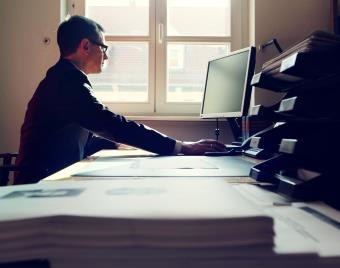
\includegraphics[width=6cm]{Abbildungen/wissen.jpg}
	\caption[Wissenschaftler an seinem Arbeitsplatz.]{Wissenschaftler an seinem Arbeitsplatz. Bilder bitte immer manuell mit dem Parameter [h] setzen. An dieser Stelle ist das Bild mit dem Figure-Parameter [h] platziert worden. Vor und nach der Figure-Umgebung steht eine Leerzeile.}
	\label{fig:wissen}
\end{figure}

Pellentesque habitant morbi tristique senectus et netus et malesuada fames ac turpis egestas. In dui magna, posuere eget, vestibulum et, tempor auctor, justo. In ac felis quis tortor malesuada pretium. Pellentesque auctor neque nec urna. Proin sapien ipsum, porta a, auctor quis, euismod ut, mi. Aenean viverra rhoncus pede. Pellentesque habitant morbi tristique senectus et netus et malesuada fames ac turpis egestas. Ut non enim eleifend felis pretium feugiat vivamus quis mi. Phasellus a est. Phasellus magna. In hac habitasse platea dictumst. Curabitur at lacus ac velit ornare lobortis.

Pellentesque habitant morbi tristique senectus et netus et malesuada fames ac turpis egestas. In dui magna, posuere eget, vestibulum et, tempor auctor, justo. In ac felis quis tortor malesuada pretium. Pellentesque auctor neque nec urna. Proin sapien ipsum, porta a, auctor quis, euismod ut, mi. Aenean viverra rhoncus pede. Pellentesque habitant morbi tristique senectus et netus et malesuada fames ac turpis egestas. Ut non enim eleifend felis pretium feugiat vivamus quis mi. Phasellus a est. Phasellus magna. In hac habitasse platea dictumst. Curabitur at lacus ac velit ornare lobortis. Pellentesque habitant morbi tristique senectus et netus et malesuada fames ac turpis egestas.

%Pellentesque habitant morbi tristique senectus et netus et malesuada fames ac turpis egestas. In dui magna, posuere eget, vestibulum et, tempor auctor. Pellentesque habitant morbi tristique senectus et netus et malesuada fames ac turpis egestas. In dui magna, posuere eget, vestibulum et, tempor auctor.

\begin{table}[h] % "\begin{table}" ist eine Umgebung für Gleitobjekte, damit die Tabelle "\begin{tabular}" nummeriert, übertitelt und mit einem Label versehen und darauf verwiesen werden kann
	\caption{Auch Tabellen ("table") werden immer mit dem Parameter [h] eingefügt. Vor und nach der Tabellen-Umgebung steht eine Leerzeile.}
	\begin{tabularx}{\textwidth}{XXXXXXXX} \toprule
		Spalte1 & Spalte2 & Spalte3 & Spalte4 & Spalte5
		& Spalte6 & Spalte7 & Spalte8 \\ \midrule
		AA      & BB      & CC      & DD      &
		EE      & FF      & GG      & HH       \\
		AA      & BB      & CC      & DD
		& EE      & FF      & GG      & HH    \\
		AA      & BB      & CC      & DD
		& EE      & FF      & GG      & HH    \\
		AA      & BB      & CC      & DD
		& EE      & FF      & GG      & HH    \\
		AA      & BB      & CC      & DD
		& EE      & FF      & GG      & HH    \\
		AA      & BB      & CC      & DD
		& EE      & FF      & GG      & HH     \\ \bottomrule
	\end{tabularx}
\end{table}

Pellentesque habitant morbi tristique senectus et netus et malesuada fames ac turpis egestas. In dui magna, posuere eget, vestibulum et, tempor auctor. Pellentesque habitant morbi tristique senectus et netus et malesuada fames ac turpis egestas. In dui magna, posuere eget, vestibulum et, tempor auctor.

% Theorie
\markboth{Theorie}{Theorie}
\chapter[Theorie (hier steht der Kurztitel im Inhaltsverzeichnis und in der Kopfzeile)]{Theorie. Hier steht der lange Titel im Fließtext, der für die Kopfzeile zu lang wäre bzw. \mbox{über zwei Zeilen laufen würde.} Manuelle Umbrüche können \mbox{mit mbox erzeugt werden}}
\label{cha:Theorie}

%%%%%%%%%%%%%%%%%%%%%%%%%%%%%%%%%%%%%%%%%%%%%%%%%%

Lorem ipsum dolor sit amet, consetetur sadipscing elitr, sed diam nonumy eirmod tempor invidunt ut labore et dolore magna aliquyam erat, sed diam voluptua. At vero eos et accusam et justo duo dolores et ea rebum. Stet clita kasd gubergren, no sea takimata sanctus est Lorem ipsum dolor sit amet. Lorem ipsum dolor sit amet, consetetur sadipscing elitr, sed diam nonumy eirmod tempor invidunt ut labore et dolore magna aliquyam erat, sed diam voluptua. At vero eos et accusam et justo duo dolores et ea rebum. Stet clita kasd gubergren, no sea takimata sanctus est Lorem ipsum dolor sit amet.

Lorem ipsum dolor sit amet, consetetur sadipscing elitr, sed diam nonumy eirmod tempor invidunt ut labore et dolore magna aliquyam erat, sed diam voluptua. At vero eos et accusam et justo duo dolores et ea rebum. Stet clita kasd gubergren, no sea takimata sanctus est Lorem ipsum dolor sit amet. Lorem ipsum dolor sit amet, consetetur sadipscing elitr, sed diam nonumy eirmod tempor invidunt ut labore et dolore magna aliquyam erat, sed diam voluptua. At vero eos et accusam et justo duo dolores et ea rebum. Stet clita kasd gubergren, no sea takimata sanctus est Lorem ipsum dolor sit amet.

Lorem ipsum dolor sit amet, consetetur sadipscing elitr, sed diam nonumy eirmod tempor invidunt ut labore et dolore magna aliquyam erat, sed diam voluptua. At vero eos et accusam et justo duo dolores et ea rebum. Stet clita kasd gubergren, no sea takimata sanctus est Lorem ipsum dolor sit amet. Lorem ipsum dolor sit amet, consetetur sadipscing elitr, sed diam nonumy eirmod tempor invidunt ut labore et dolore magna aliquyam erat, sed diam voluptua. At vero eos et accusam et justo duo dolores et ea rebum. Stet clita kasd gubergren, no sea takimata sanctus est Lorem ipsum dolor sit amet.

\begin{table}[h] % "\begin{table}" ist eine Umgebung für Gleitobjekte, damit die Tabelle "\begin{tabular}" nummeriert, übertitelt und mit einem Label versehen und darauf verwiesen werden kann
	\caption[Od quo tecto offic torit eteum acerum fuga. Ideni omnihic idundero doluptus iminvel luptati busdaepta sequi dolorec tatessinum.]{Auch Tabellen ("table") werden immer mit dem Parameter [h] eingefügt. Vor und nach der Tabellen-Umgebung steht eine Leerzeile. Fügen sie mit "newline" manuelle Zeilenumbrüche ein, wenn die Abstände zwischen den Wörtern in einer Zelle zu groß werden.}
	\centering
	\begin{tabular}{ | l | l | l | p{2.5cm} |}
			\hline
			Aliquyam & Dolor & Rebum & Sadipscing \\ \hline
			Invidunt & Labore & Sanctus & Stet clita kasd \newline gubergren. \\ \hline
			Magna & Gubergren & Clita & No sea takimata \newline sanctus. \\ \hline
			Eirmod & Voluptua & Aliquyam & Sed diam nonumy eirmod tempor. \\
			\hline%
	\end{tabular}%
	\label{tab:tab}%
\end{table}%

Od quo tecto offic torit eteum acerum fuga. Ideni omnihic idundero doluptus iminvel luptati busdaepta sequi dolorec tatessinum quas et quia perae et qui blanditi quiberit alique provit, cus incipid ut quis enis vel id es asperum volor aut unt, quatum eturem aciassin et rest inulluptam et volecae. Od quo tecto offic torit eteum acerum fuga. Ideni omnihic idundero doluptus iminvel luptati busdaepta sequi dolorec tatessinum quas et quia perae et qui blanditi quiberit alique provit, cus incipid ut quis enis vel id es asperum volor aut unt, quatum eturem aciassin et rest inulluptam et volecae. Od quo tecto offic torit eteum acerum fuga. Ideni omnihic idundero doluptus iminvel luptati busdaepta sequi dolorec tatessinum quas et quia perae et qui blanditi quiberit alique provit, cus incipid ut quis enis vel id es asperum volor aut unt, quatum eturem aciassin et rest inulluptam et volecae. Od quo tecto offic torit eteum acerum fuga. Ideni omnihic idundero doluptus iminvel luptati busdaepta sequi dolorec tatessinum quas et quia perae et qui blanditi quiberit alique provit, cus incipid ut quis enis vel id es asperum volor aut unt, quatum eturem aciassin et rest inulluptam et volecae.
\begin{subequations}
	\label{maxwell-gleichungen}
	\begin{align}
	\text{div }(\vec{D}) &= 4 \cdot \pi \cdot \rho
	\label{coulomb-gesetz}\\
	\text{rot }(\vec{H}) &= \frac{4 \cdot \pi}{c} \cdot \vec{j}
	\label{ampere-gesetz}\\
	\text{rot }(\vec{E}) &= - \frac{1}{c} \cdot \frac{\partial \vec{B}}{\partial t}
	\label{faraday-gesetz-1} \\
	\text{div }(\vec{B}) &= 0
	\label{faraday-gesetz-2}
	\end{align}
\end{subequations}
Arepelisti re denda doluptata quo demque conseribeate eum quiberor aut quatur maiorae riberis eserio eaturepro ommo bero eum que quisquidit volendis eni asi sint aut pe minis is re nonseque ius aut pa is expel ium nobis miliquati dolupit, qui nullanis re, sitiis si volor mo te eventia vendit qui dolupta quamusda vereped magnihi cturem dendignatus vite prernatatis soluptat aperum sequostorum et quistru pienitiis arum, optaquo qui comnis cuptam qui officitate pellent ariae occaborrovid mod esequi dolorum rerro quas vent harciistia quis voloris sinctiis ea nistrum facius simus utem sit, inctor sit dolorrum ditio. Ecerum et est quia doluptur? Qui dolorero des nosapis exerias dest, qui coratur itemporum repeliq uiassit, inum fugiasi simil est alicium ilis que nimusanis es suntiaestrum ium ium harcil iligent excearum fugia nonsequia dem.
% Binomialkoeffizient:
\begin{align*}
\binom{n}{k} = \frac{n!}{(n - k)! \cdot k!}
\end{align*}
Optaquo qui comnis cuptam qui officitate pellent ariae occaborrovid mod esequi dolorum rerro quas vent harciistia quis voloris sinctiis ea nistrum facius simus utem sit, inctor sit dolorrum ditio. Ecerum et est quia doluptur? Qui dolorero des nosapis exerias dest, qui coratur itemporum repeliq uiassit, inum fugiasi simil est alicium ilis que nimusanis es suntiaestrum ium ium harcil iligent excearum fugia nonsequia dem.
\begin{equation} 
\prod \limits_{i=1}^{n+1}i = 1\cdot 2\cdot\dots\cdot n\cdot (n+1) \
\end{equation}
Arepelisti re denda doluptata quo demque conseribeate eum quiberor aut quatur maiorae riberis eserio eaturepro ommo bero eum que quisquidit volendis eni asi sint aut pe minis is re nonseque ius aut pa is expel ium nobis miliquati dolupit, qui nullanis re, sitiis si volor mo te eventia vendit qui dolupta quamusda vereped magnihi cturem dendignatus vite prernatatis soluptat aperum sequostorum et quistru pienitiis arum, optaquo qui comnis cuptam qui officitate pellent ariae occaborrovid mod esequi dolorum rerro quas vent harciistia quis voloris sinctiis ea nistrum facius simus utem sit, inctor sit dolorrum ditio. Ecerum et est quia doluptur? Qui dolorero des nosapis exerias dest, qui coratur itemporum repeliq uiassit, inum fugiasi simil est alicium ilis que nimusanis es suntiaestrum ium ium harcil iligent excearum fugia nonsequia dem. Ovidus.

% Zusammenfassung und Ausblick
\markboth{Zusammenfassung und Ausblick}{Zusammenfassung und Ausblick}
\chapter{Zusammenfassung und Ausblick}
\label{cha:Zusammenfassung und Ausblick}

%%%%%%%%%%%%%%%%%%%%%%%%%%%%%%%%%%%%%%%%%%%%%%%%%%

\section{Zusammenfassung}
\label{sec:Zusammenfassung}
Arepelisti re denda doluptata quo demque conseribeate eum quiberor aut quatur maiorae riberis eserio eaturepro ommo bero eum que quisquidit volendis eni asi sint aut pe minis is re nonseque ius aut pa is expel ium nobis miliquati dolupit, qui nullanis re, sitiis si volor mo te eventia vendit qui dolupta quamusda vereped magnihi cturem dendignatus vite prernatatis soluptat aperum sequostorum et quistru pienitiis arum, optaquo qui comnis cuptam qui officitate pellent ariae occaborrovid mod esequi dolorum rerro quas vent harciistia quis voloris sinctiis ea nistrum facius simus utem sit, inctor sit dolorrum ditio. Ecerum et est quia doluptur? Qui dolorero des nosapis exerias dest, qui coratur itemporum repeliq uiassit, inum fugiasi simil est alicium ilis que nimusanis es suntiaestrum ium ium harcil iligent excearum fugia nonsequia dem.

Arepelisti re denda doluptata quo demque conseribeate eum quiberor aut quatur maiorae riberis eserio eaturepro ommo bero eum que quisquidit volendis eni asi sint aut pe minis is re nonseque ius aut pa is expel ium nobis miliquati dolupit, qui nullanis re, sitiis si volor mo te eventia vendit qui dolupta quamusda vereped magnihi cturem dendignatus vite prernatatis soluptat aperum sequostorum et quistru pienitiis arum, optaquo qui comnis cuptam qui officitate pellent ariae occaborrovid mod esequi dolorum rerro quas vent harciistia quis voloris sinctiis ea nistrum facius simus utem sit, inctor sit dolorrum ditio. Ecerum et est quia doluptur? Qui dolorero des nosapis exerias dest, qui coratur itemporum repeliq uiassit, inum fugiasi simil est alicium ilis que nimusanis es suntiaestrum ium ium harcil iligent excearum fugia nonsequia dem.

\section{Ausblick}
\label{sec:Ausblick}
Arepelisti re denda doluptata quo demque conseribeate eum quiberor aut quatur maiorae riberis eserio eaturepro ommo bero eum que quisquidit volendis eni asi sint aut pe minis is re nonseque ius aut pa is expel ium nobis miliquati dolupit, qui nullanis re, sitiis si volor mo te eventia vendit qui dolupta quamusda vereped magnihi cturem dendignatus vite prernatatis soluptat aperum sequostorum et quistru pienitiis arum, optaquo qui comnis cuptam qui officitate pellent ariae occaborrovid mod esequi dolorum rerro quas vent harciistia quis voloris sinctiis ea nistrum facius simus utem sit, inctor sit dolorrum ditio. Ecerum et est quia doluptur? Qui dolorero des nosapis exerias dest, qui coratur itemporum repeliq uiassit, inum fugiasi simil est alicium ilis que nimusanis es suntiaestrum ium ium harcil iligent excearum fugia nonsequia dem.



% Schlussfolgerungen und Ausblick
%\include{Inhalt/07_Schlussfolgerungen_und_Ausblick}

%%%%%%%%%%%%%%%%%%%%%%%%%%%%%%%%%%%%%%%%%%%%%%%%%%
%%%				Anhang (include)	 		   %%%
%%%%%%%%%%%%%%%%%%%%%%%%%%%%%%%%%%%%%%%%%%%%%%%%%%

% Anhang; Kapitel im Anhang erhalten Großbuchstaben im Inhaltsverzeichnis
\appendix 

\markboth{Anhang}{Anhang}
\chapter{Anhang}
\label{cha:Anhang}

%%%%%%%%%%%%%%%%%%%%%%%%%%%%%%%%%%%%%%%%%%%%%%%%%%

Lorem ipsum dolor sit amet, consetetur sadipscing elitr, sed diam nonumy eirmod tempor invidunt ut labore et dolore magna aliquyam erat, sed diam voluptua. At vero eos et accusam et justo duo dolores et ea rebum. Stet clita kasd gubergren, no sea takimata sanctus est Lorem ipsum dolor sit amet. Lorem ipsum dolor sit amet, consetetur sadipscing elitr, sed diam nonumy eirmod tempor invidunt ut labore et dolore magna aliquyam erat, sed diam voluptua. At vero eos et accusam et justo duo dolores et ea rebum. Stet clita kasd gubergren, no sea takimata sanctus est Lorem ipsum dolor sit amet.

%%%%%%%%%%%%%%%%%%%%%%%%%%%%%%%%%%%%%%%%%%%%%%%%%%
%%%				Verzeichnisse (include)		   %%%
%%%%%%%%%%%%%%%%%%%%%%%%%%%%%%%%%%%%%%%%%%%%%%%%%%

% Abbildungsverzeichnis
\listoffigures

% Tabellenverzeichnis
\listoftables

% Literaturverzeichnis
\markboth{Literaturverzeichnis}{Literaturverzeichnis}

%%%%%%%%%%%%%%%%%%%%%%%%%%%%%%%%%%%%%%%%%%%%%%%%%%

\chapter*{Eigene Veröffentlichungen}
\addcontentsline{toc}{chapter}{Eigene Veröffentlichungen}

\section*{Journalartikel}
\addcontentsline{toc}{section}{Journalartikel}
\renewcommand{\refnamejournal}{Journalartikel}
\begingroup % Überschrift von \bibliography{} löschen
\renewcommand{\chapter}[2]{}
\renewcommand{\section}[2]{}
\nocitejournal{*} % Alle Titel der .bib-Datei im Literaturverzeichnis anzeigen, wenn aktiviert; bei Deaktivierung werden nur die zitierten Titel angezeigt
\bibliographystylejournal{plainnat}
\bibliographyjournal{Literatur/Eigene_Journal_Papers}{}
\endgroup

%%%%%%%%%%%%%%%%%%%%%%%%%%%%%%%%%%%%%%%%%%%%%%%%%%

\section*{Konferenzbeitr\"age}
\addcontentsline{toc}{section}{Konferenzbeiträge}
\renewcommand{\refnameconference}{Konferenzbeiträge}
\begingroup % Überschrift von \bibliography{} löschen
\renewcommand{\chapter}[2]{}
\renewcommand{\section}[2]{}
\nociteconference{*} % Alle Titel der .bib-Datei im Literaturverzeichnis anzeigen, wenn aktiviert; bei Deaktivierung werden nur die zitierten Titel angezeigt
\bibliographystyleconference{plainnat}
\bibliographyconference{Literatur/Eigene_Konferenz_Papers}{}
\endgroup

%%%%%%%%%%%%%%%%%%%%%%%%%%%%%%%%%%%%%%%%%%%%%%%%%%

\chapter*{Literaturverzeichnis}
\addcontentsline{toc}{chapter}{Literaturverzeichnis}
\renewcommand{\refname}{Literaturverzeichnis}
\renewcommand\bibname{Literaturverzeichnis}
\begingroup % Überschrift von \bibliography{} löschen
\renewcommand{\chapter}[2]{}
\renewcommand{\section}[2]{}
\nocite{*} % Alle Titel der .bib-Datei im Literaturverzeichnis anzeigen, wenn aktiviert; bei Deaktivierung werden nur die zitierten Titel angezeigt
\bibliographystyle{plainnat} % Zitierstil bei Bedarf anpassen
\bibliography{Literatur/Externe_Literatur}{}
\endgroup

%%%%%%%%%%%%%%%%%%%%%%%%%%%%%%%%%%%%%%%%%%%%%%%%%%

%\markboth{Literaturverzeichnis}{Literaturverzeichnis}
%\renewcommand{\refname}{Literaturverzeichnis}
%\renewcommand\bibname{Literaturverzeichnis}
%\bibliography{Literatur/Eigene_Konferenz_Papers}{}
%\bibliographystyle{alpha}
%\nocite{*}

% Setzt Kapitelüberschrift auch auf rechte Seite der Kopfzeile, da keine Unterkapitel
\renewcommand{\chaptermark}[1]{\markboth{\thechapter\ \  #1}{\thechapter\ \  #1}} 

% Änderung der Abstände zwischen den Einträgen
\setlength{\parskip}{0.3\baselineskip plus 0.15\baselineskip minus 0.15\baselineskip} 

\end{document}